\documentclass[a4paper]{article}
\usepackage{amsmath}
\usepackage{graphicx}
\usepackage{xcolor}
\usepackage{pgfplots}
\usepackage{subcaption} % Package for managing subfigures
\usepackage{url}

\title{Transforming Images with Transfer Functions: Enhancing Medical Imaging for Brain Tumor Detection}
\author{Jakub Vlk$^{1,2}$ \\ Manuel G. Forero$^2$ }
\date{}

\begin{document}

\maketitle

\begin{center}
    
\quad $^1$ Brno University of Technology \\
\quad $^2$ Semillero L{\'{u}}n -- Universidad de Ibagué
\end{center}

\section{Introduction}

In medical imaging, the accurate and clear visualization of the brain is crucial for detecting diseases. One advanced technique employed to enhance medical images involves the use of transfer functions. This article explores the application of transfer functions, specifically the sigmoid and hyperbolic tangent functions, to transform medical images, thereby improving the visibility of brain tumors.

\section{Transfer Functions in Medical Imaging}

Transfer functions are mathematical functions that create a table (LUT) specifying how to transform every pixel in the image. In medical imaging, transfer functions manipulate the intensity values of pixels to improve contrast and highlight areas of interest. For the brain, the goal is to increase the differentiation of gray colors, making it easier to identify different parts of the brain. This process is beneficial for identifying and delineating brain tumors, which may be difficult to detect in raw images due to their subtle differences in intensity compared to surrounding tissues.

\begin{figure}
  \centering
    \begin{subfigure}[b]{0.4\textwidth}
        \centering
        \includegraphics[width=\textwidth]{IRM072_2.jpg}
        \caption{Original}
        \label{fig:sub1}
    \end{subfigure}
    \begin{subfigure}[b]{0.4\textwidth}
        \centering
        \includegraphics[width=\textwidth]{IRM072_tran.jpg}
        \caption{Transformed}
        \label{fig:sub2}
    \end{subfigure}
\end{figure}

\section{The Role of the Sigmoid Function}

The sigmoid function, defined as:
\begin{equation}
f(x) = \frac{1}{1 + e^{-x}},
\end{equation}
is an S-shaped curve that maps any real-valued number into the range $(0,1)$. This function is particularly useful in medical imaging for its ability to stretch the intensity values of pixels in a nonlinear manner, thereby enhancing the contrast between different tissues.

To adapt the sigmoid function for image transformation, it is scaled to the intensity range of the image. The function is in the range of $(0,1)$, so it can be transformed to any range by multiplication. In terms of input value, the function is changed so that $f(0) \approx 0$ and $f(1) \approx 1$.
\begin{equation}
\label{transformedSigmoid}
f(x) = \frac{1}{1 + e^{-2 \cdot \ln(255) \cdot \left(\frac{x}{255} - 0.5\right)}}
\end{equation}

\begin{figure}[h!]
\centering
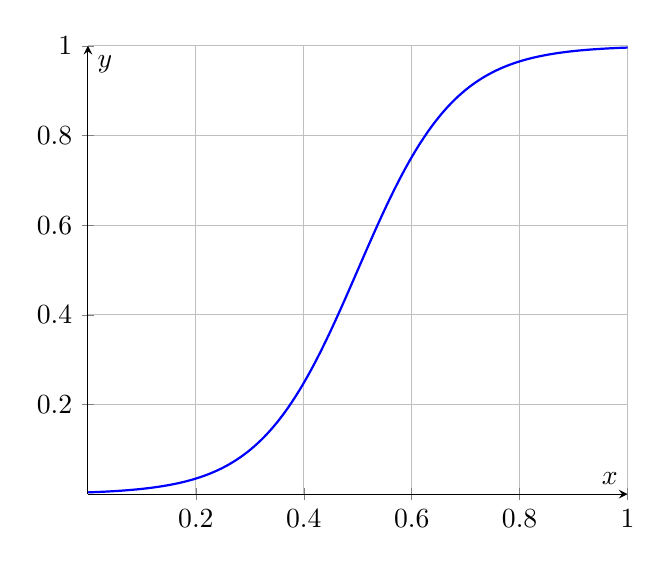
\begin{tikzpicture}[scale=1]
  \begin{axis}[
    grid=both, % Activate grid
    axis lines=middle, % Draw axes in the middle of the graph
    enlargelimits=false, % Do not add extra space around the graph
    xlabel={$x$}, % Label for x-axis
    ylabel={$y$}, % Label for y-axis
    xmin=0, xmax=1, % Limit range for x-axis
    ymin=0, ymax=1, % Limit range for y-axis
    xtick={0, 0.2, 0.4, 0.6, 0.8, 1}, % Grid intervals on x-axis
    ytick={0, 0.2, 0.4, 0.6, 0.8, 1} % Grid intervals on y-axis
  ]
    
    \addplot [
        domain=-0.1:1.1, 
        samples=1000, 
        thick, 
        blue
    ] 
    {1 / (1 + exp(-2 * ln(255) * (x - 0.5)))};
    \end{axis}
\end{tikzpicture}
\caption{Scaled sigmoid function }
\end{figure}

\section{The Hyperbolic Tangent Function}

Another effective transfer function is the hyperbolic tangent, defined as:
\begin{equation}
\tanh(x) = \frac{e^x - e^{-x}}{e^x + e^{-x}}.
\end{equation}
Similar to the sigmoid function, the hyperbolic tangent maps real-valued inputs to a specific range, in this case $(-1, 1)$.

For image processing, the hyperbolic tangent function can be scaled to fit the intensity range of the image:
\begin{equation}
f(x) = \frac{\tanh(6x-3)+1}{2} 
\end{equation}

\begin{figure}[h!]
\centering
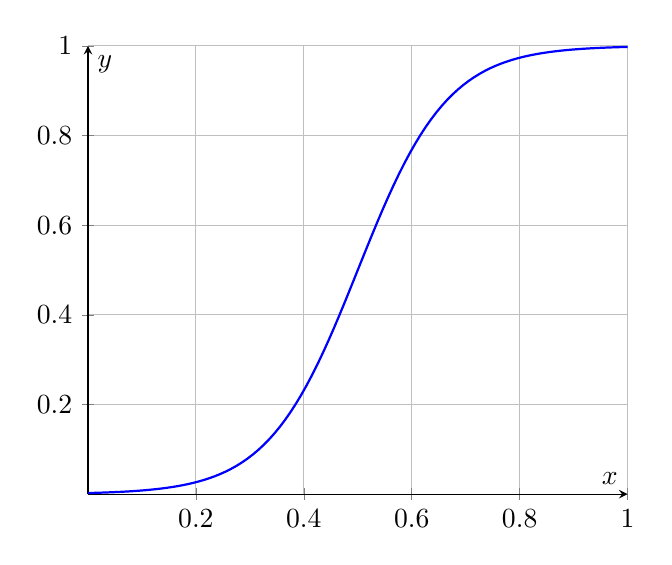
\begin{tikzpicture}[scale=1]
  \begin{axis}[
    grid=both, % Activate grid
    axis lines=middle, % Draw axes in the middle of the graph
    enlargelimits=false, % Do not add extra space around the graph
    xlabel={$x$}, % Label for x-axis
    ylabel={$y$}, % Label for y-axis
    xmin=0, xmax=1, % Limit range for x-axis
    ymin=0, ymax=1, % Limit range for y-axis
    xtick={0, 0.2, 0.4, 0.6, 0.8, 1}, % Grid intervals on x-axis
    ytick={0, 0.2, 0.4, 0.6, 0.8, 1} % Grid intervals on y-axis
  ]
    
    \addplot [
        samples=1000, 
        thick, 
        blue
    ] 
    {(tanh(6*x-3) + 1) /2};
    \end{axis}
\end{tikzpicture}
\caption{Hyperbolic tangent function scaled for image intensity range}
\end{figure}

\section{Usage}

A plugin for ImageJ was developed for the application of these functions\footnote{Source code can be found at \url{https://github.com/vlccek/imagej_contrast_stretching}}. The function can be edited or completely redefined.

\begin{figure}[h!]
    \centering
    \includegraphics[width=1.1\linewidth]{plugin.png}
    \caption{Developed plugin}
    \label{fig:enter-label}
\end{figure}

\end{document}
